% concatenated from log-concavity-rows-super-recurrence.tex
\documentclass{article}
\usepackage[utf8]{inputenc}
\usepackage[babel]{microtype}
\usepackage[english]{babel}
\usepackage{fullpage}
% \usepackage{quiver}
\usepackage{comment}

%%%% Math packages
\usepackage{amsmath,amssymb,amsthm, mathrsfs, mathtools,bbm,bm}
\usepackage[usenames,dvipsnames]{xcolor}
\usepackage{multirow}
\usepackage{tikz-cd,tikz}
\usetikzlibrary{arrows.meta, positioning}
\usetikzlibrary{decorations.pathreplacing, calligraphy}
%%%% Lists
\usepackage{enumitem}
\setlist[enumerate,1]{label={(\roman*)}}%,noitemsep, topsep=0pt}
\setlist[enumerate,2]{label={(\alph*)}}%,noitemsep, topsep=0pt}
\setlist[enumerate,3]{label={(\arabic*)}}%,noitemsep, topsep=0pt}
%\setlist[itemize]{nolistsep,noitemsep, topsep=0pt}
\tikzcdset{scale cd/.style={every label/.append style={scale=#1},
    cells={nodes={scale=#1}}}}
%%%% Hyperlinks
\usepackage[hypertexnames=false]{hyperref}
\hypersetup{
    colorlinks,
    linkcolor={red!60!black},
    citecolor={green!60!black},
    urlcolor={blue!60!black}
}

%%%% Math letters
\newcommand{\mc}[1]{\ensuremath{\mathcal #1}}
\newcommand{\bb}[1]{\ensuremath{\mathbb #1}}
\newcommand{\dd}{\mathcal{D}}
\newcommand{\lp}{\mathcal{P}}
\newcommand{\SSS}{\mathfrak{S}}
\newcommand{\eul}{\mathcal{A}}
\newcommand{\tl}{\mathtt{1}} 
\newcommand{\tO}{\mathtt{0}}
\newcommand{\occ}[2]{N^{#1}(#2)}
\newcommand{\occempty}[1]{N^{#1}}
\newcommand{\fl}[1]{\left\lfloor #1 \right\rfloor}
\newcommand{\N}{\mathbb{N}}
\newcommand{\Z}{\mathbb{Z}}
\newcommand{\R}{\mathbb{R}}
\newcommand{\C}{\mathbb{C}}
\newcommand{\dens}{\operatorname{dens}}




\DeclareMathOperator{\e}{e}     % exp(ix)

\DeclareMathOperator{\LandauO}{\mathcal O}             % Big O-notation
\DeclareMathOperator{\realpart}{\mathrm {Re}}
\DeclareMathOperator{\imagpart}{\mathrm{Im}}
\DeclareMathOperator{\pr}{psn}
\DeclareMathOperator{\wt}{wt}
\DeclareMathOperator{\im}{Im}
\DeclareMathOperator{\ch}{ch}
\DeclareMathOperator{\cl}{cl}
\DeclareMathOperator{\rev}{rev}
\DeclareMathOperator{\bl}{bl}

\DeclarePairedDelimiter{\parens}{(}{)}
%\newcommand{\cum}{\kappa}
%\def\bl{\hspace{0.5pt}\underline{\hphantom{\hspace{0.6em}}}\hspace{0.5pt}}	%bottom line
%\newcommand{\gammap}{\gamma^*}


\newtheorem{customproposition}{Proposition}
\newenvironment{customprop}[1]
  {\renewcommand\thecustomproposition{#1}\customproposition}
  {\endcustomproposition}

\newtheorem{theorem}{Theorem}[section]
\newtheorem{proposition}[theorem]{Proposition}
\newtheorem{corollary}[theorem]{Corollary}
\newtheorem{lemma}[theorem]{Lemma}
\newtheorem{conjecture}[theorem]{Conjecture}

\theoremstyle{definition}
\newtheorem*{remark}{Remark}
\newtheorem{example}{Example}
\numberwithin{equation}{section}
 
\usepackage{authblk}
\title{Log-concavity of rows of triangular arrays satisfying a certain super-recurrence}
\author[1]{Umesh Shankar\thanks{\tt{204093001@iitb.ac.in, umeshshankar@outlook.com}}} 
\affil[1]{Department of Mathematics, Indian Institute of Technology Bombay, Mumbai 400076, India} 
\date{\today}
\begin{document}
\maketitle
\begin{abstract}
Recurrences of the form 
\begin{equation*}
    T(n,k) = (\alpha n+\beta k +\gamma) \ T(n-1,k) + (\alpha'n+\beta'k+\gamma')\ T(n-1,k-1)+\delta_{n,0}\delta_{k,0}.
\end{equation*}
show up as the recurrence for many well-studied combinatorial sequences such as the Stirling numbers of first and second kind, the Lah numbers, Eulerian numbers etc. Recently, many of these sequences have received generalisations that obey a recurrence of the form
\begin{equation*}
    T(n,k) = (\alpha n+\beta k +\gamma)^l \ T(n-1,k) + (\alpha'n+\beta'k+\gamma')^l\ T(n-1,k-1)+\delta_{n,0}\delta_{k,0}.
\end{equation*}
where $l$ is a positive integer. Many of these generalised sequences also satisfy properties such as unimodality, log-concavity, gamma-nonnegativity, real-rootedness that the original sequences satisfy. In this article, we give sufficient conditions for rows of triangular arrays, arising from the recurrence stated above, to be log-concave. We show that our sufficient condition is satisfied by many of the classical examples, thereby giving a new unified approach to proving their log-concavity. This sufficient condition also confirms a conjecture of Tankosi{\v c} \cite{aleks-gen-lah} about the log-concavity of generalised Lah numbers. 

Our main technique will be to interpret the triangular array $(T(n,k))$ as weighted lattice paths and produce an injection that is increasing in weight.
Finally, we introduce a two-parameter generalisation of the Eulerian numbers analogous to the generalised Stirling and Lah counterparts. We prove that this sequence is palindromic and make some remarks about their gamma-nonnegativity and real-rootedness.
\end{abstract}
% \textbf{\small{}Keyword:}{\small{} }{\let\thefootnote\relax\footnotetext{The author is supported by the National Board for Higher Mathematics, India.}}{\let\thefootnote\relax\footnotetext{2020 \textit{Mathematics Subject Classification}. Primary ; 
% Secondary , .}}
\section{Introduction}
Let $\N$ denote the set of non-negative integers and for $n \in \N$, let $[n]$ denote the set $\{ 1,2,\dotsc, n\}$. A finite sequence of real numbers $(a_k)_{k=0}^n$ is said to be log-concave if $a_{k}^2\ge a_{k+1}a_{k-1}$ for all indices $k\in [n-1]$. Log-concavity is a well-studied property of finite sequences and it appears in various areas of mathematics such as combinatorics, probability and algebra. See the surveys of Stanley \cite{stanley-survey-logcon}, Branden \cite{branden-unimodality_log_concavity} for a wealth of results on log-concavity.
% Let $\SSS_n$ denote the set of permutations of $[n]$.

A \emph{triangular array} $T(n,k)$ is a collection of real numbers that satisfies a recurrence of the form 
\begin{equation}\label{Eq:triangular}
    T(n,k) = c(n,k)\ T(n-1,k) + d(n,k)\ T(n-1,k-1) + \delta_{n,0}\delta_{k,0}, \qquad \text{for }n, k \geq 0,
\end{equation}
and $T(n,k) = 0$ for $n < 0$, $k < 0$, or $k > n$, for some $c(n,k), d(n,k) \in \mathbb{R}$ and $\delta_{i,j}$ is the Kronecker delta function.
Several interesting enumerative sequences obey a recurrence of this form, including the binomial numbers, $\binom{n}{k}$, the Stirling numbers of the first and second kinds, $s(n,k)$ and $S(n,k)$, the Lah numbers, $L(n,k)$, and the Eulerian numbers, $A(n,k)$.
These sequences and their generating functions are rich in combinatorial structure, and well-studied in the literature, in particular with respect to properties such as log-concavity, unimodality, gamma positivity, and real-rootedness.
Moreover, in all these examples we have that the expressions for $c(n,k)$ and $d(n,k)$ are affine functions in the variables $n$ and $k$.

% {\color{red}{(I think the point I wanted to highlight by the last remark is that we know log concavity for triangular arrays in which the coefficients are of a certain kind, but those methods do not generalize when that form changes; yet, the methods of this paper work uniformly for the simpler and more complicated recurrences, both. This has to be said somewhere in the introduction. Maybe somewhere in the intro you could mention Sagan's theorem (I think?) and note that it does not help for the generalized Stirling and Lah numbers, and those needed different methods.}}

To prove the log-concavity of the Stirling numbers of both kinds, Kurtz \cite{kurtz-log-concavity} gave the following sufficient condition for triangular arrays.

\begin{theorem}[{\cite[Theorem 2]{kurtz-log-concavity}}]
    Let $T(n,k)=c(n,k)\ T(n-1,k) + d(n,k)\ T(n-1,k-1)$ and 
    \begin{itemize}
        \item $2c(n,k)\ge c(n,k-1)+c(n,k+1),$
        \item $2d(n,k)\ge d(n,k-1)+d(n,k+1),$
    \end{itemize}
     then, the array $T(n,k)$ is log-concave in $k$, for all $n$.
\end{theorem}
% \end{frame}

A strengthening of the Theorem was obtained by Sagan \cite{sagan-log-concave} wherein the hypothesis of concavity of the coefficients was weakened to log-concavity of the coefficients and concavity of the product. The theorem is as follows.

\begin{theorem}[{\cite[Theorem 1]{sagan-log-concave}}]
    Let $T(n,k)$ be an extended triangular array satisfying $T(n,k)=c(n,k)\ T(n-1,k) + d(n,k)\ T(n-1,k-1)$ for all $n\ge 1$ and $T(n,k),c(n,k),d(n,k)$ are all non-negative integers. Suppose 
    \begin{itemize}
        \item $c(n,k),d(n,k)$ are log-concave in $k$,
        \item $d(n,k-1)c(n,k+1)+d(n,k+1)c(n,k-1)\le 2d(n,k)c(n,k)$,
    \end{itemize}
    then, the $T(n,k)$ are log-concave in $k$.
\end{theorem}

Recently, some of the enumerative sequences listed above have been generalized by introducing more parameters.
Let $r \in \N$.The \index{$r$-Stirling number of the first kind}$r$-Stirling number of the first kind, $s_r(n,k)$ (with $n\ge k\ge r$), is defined to be the number of permutations 
in $\SSS_n$ with $k$ cycles such that $1,2,\dotsc, r$ are in different cycles.
The \index{$r$-Stirling number of the second kind}$r$-Stirling number of the second kind, $S_r(n,k)$ (with $n\ge k\ge r$), is defined to be the number of partitions
 of $[n]$ into $k$ blocks such that $1,2,\dots,r$ are in different blocks. These numbers have been studied in great detail, see \cite{broder-r-stir, stirling-ref-2}.
The closely related\index{$r$-Lah number} $r$-Lah number, $L_r(n,k)$ (with $n\ge k\ge r$), is defined to be the number of partitions of 
$[n]$ into $k$ nonempty ordered subsets such that $1,2,\dots,r$ are in different ordered subsets.
These were studied in \cite{r-lah-ref-1,r-lah-ref-2,lah-ref-3}.
The $r$-Stirling numbers and $r$-Lah numbers are also triangular arrays in the sense of \eqref{Eq:triangular}, with 
coefficients that are affine functions in the variables.

These numbers have been further generalised with an additional parameter as follows (see \cite{lr-stir-ref,aleks-gen-lah}).
Let $l \in \mathbb{N}$.
Define the \index{cycle leader}\emph{cycle leader} of a permutation $\pi \in \SSS_n$, denoted $\cl(\pi)$, to be the set of minimum elements 
of each cycle in the cycle decomposition of $\pi$.
The $(l,r)$-Stirling number of the first kind, $s_r^{(l)}(n,k)$, is defined to be the number of $l$-tuples of permutations
 $(\pi_1,\dotsc,\pi_l)$ such that $[r]\subset \cl(\pi_1)$ and $\cl(\pi_1)=\dotsb=\cl(\pi_l)$. 
Define the\index{block leader} \emph{block leader} of a partition $\Pi$ of $[n]$, denoted $\bl(\Pi)$, to be the set of minimum elements of each
 block of the partition $\Pi$.
The $(l,r)$-Stirling number of the second kind, $S_r^{(l)}(n,k)$, is defined similarly: it is the number of $l$-tuples of 
partitions $(\Pi_1,\dotsc,\Pi_l)$ such that $[r]\subset \bl(\Pi_1)$ and $\bl(\Pi_1)=\dotsb=\bl(\Pi_l)$. 
The $(l,r)$-Lah number is defined in a similar manner to the $(l,r)$-Stirling number of the second kind.
It counts the number of $l$-tuples of partitions $(\Pi_1,\dotsc,\Pi_l)$ into $k$ linearly ordered blocks such 
that $[r]\subset \bl(\Pi_1)$ and $\bl(\Pi_1)=\dotsb=\bl(\Pi_l)$.



% The $r$-Stirling number of the first kind, $s_r(n,k)$ (with $n\ge k\ge r$), is defined to be the number of permutations in $\SSS_n$ with $k$ cycles such that $1,2,\dotsc, r$ are in different cycles.
% The $r$-Stirling number of the second kind, $S_r(n,k)$ (with $n\ge k\ge r$), is defined to be the number of partitions of $[n]$ into $k$ blocks such that $1,2,\dots,r$ are in different blocks. These numbers have been studied in great detail, see \cite{}.
% The closely related $r$-Lah number, $L_r(n,k)$ (with $n\ge k\ge r$), is defined to be the number of partitions of $[n]$ into $k$ nonempty ordered subsets such that $1,2,\dots,r$ are in different ordered subsets.
% These were studied in \cite{}.
% The $r$-Stirling numbers and $r$-Lah numbers are also triangular arrays in the sense of \eqref{Eq:triangular}, with coefficients that are affine functions in the variables.

% These numbers have been further generalised with an additional parameter as follows.
% Let $l \in \mathbb{N}$.
% Define the \emph{cycle leader} of a permutation $\pi \in \SSS_n$, denoted $\cl(\pi)$, to be the set of minimum elements of each cycle in the cycle decomposition of $\pi$.
% The $(l,r)$-Stirling number of the first kind, $s_r^{(l)}(n,k)$, is defined to be the number of $l$-tuples of permutations $(\pi_1,\dotsc,\pi_l)$ such that $[r]\subset \cl(\pi_1)$ and $\cl(\pi_1)=\dotsb=\cl(\pi_l)$. 
% Define the \emph{block leader} of a partition $\Pi$ of $[n]$, denoted $\bl(\Pi)$, to be the set of minimum elements of each block of the partition $\Pi$.
% The $(l,r)$-Stirling number of the second kind, $S_r^{(l)}(n,k)$, is defined similarly: it is the number of $l$-tuples of partitions $(\Pi_1,\dotsc,\Pi_l)$ such that $[r]\subset \bl(\Pi_1)$ and $\bl(\Pi_1)=\dotsb=\bl(\Pi_l)$. 
% The $(l,r)$-Lah number is defined in a similar manner to the $(l,r)$-Stirling number of the second kind.
% It counts the number of $l$-tuples of partitions $(\Pi_1,\dotsc,\Pi_l)$ into $k$ linearly ordered blocks such that $[r]\subset \bl(\Pi_1)$ and $\bl(\Pi_1)=\dotsb=\bl(\Pi_l)$.

The $(l,r)$-Stirling numbers and $(l,r)$-Lah numbers are also triangular arrays; in particular, equation~\eqref{Eq:triangular} for these numbers take the following forms:
\begin{align*}
    s_r^{(l)}(n,k) &= (n-1)^l s_r^{(l)}(n-1,k) + s_r^{(l)}(n-1,k-1)\\
    S_r^{(l)}(n,k) &= k^l S_r^{(l)}(n-1,k) + S_r^{(l)}(n-1,k-1)\\
    L_r^{(l)}(n,k) &= (n+k-1)^l L_r^{(l)}(n-1,k) + L_r^{(l)}(n-1,k-1)
\end{align*}
for $1 \leq r \leq k \leq n$.
While it is easy to show that the $(l,r)$-Stirling numbers of both kinds are log-concave, it was conjectured in \cite{aleks-gen-lah} that the $(l,r)$-Lah numbers are log-concave in $k$ as well. However, the theorems of Kurtz and Sagan are not applicable to these arrays when $l\ge 2$. 

Motivated by the form of the recurrences appearing in the conjecture, we develop a general method to establish log-concavity of many so-called ``super-recurrence'' relations of the form
\begin{equation}\label{Eq:super-recurrence}
    T(n,k)=(\alpha n+\beta k +\gamma)^l\ T(n-1,k) + (\alpha'n+\beta'k+\gamma')^l\ T(n-1,k-1) + \delta_{n,0}\delta_{k,0}, \quad \text{for } n, k \geq 0,
\end{equation}
and $T(n,k) = 0$ for $n < 0$, $k < 0$, or $k > n$, where $\alpha,\alpha',\beta,\beta',\gamma,\gamma' \in \N$, and $\delta_{i,j}$ is the Kronecker delta function. We also show that 
The main result of the paper is a sufficient condition for log-concavity of triangular arrays which is the following.
% {\color{blue}{Insert main theorem statement here?}}
\begin{theorem}\label{thm: main}
     For $n\ge 1$ and $0<k \le n$, let $T(n,k)$ satisfy the following triangular recurrence.
    \begin{equation*}
        T(n,k)=c(n,k)\ T(n-1,k)+d(n,k)\ T(n-1,k-1)
    \end{equation*}
    The sequence $(T(n,k))_{k=0}^n$ is log-concave if $(i),(ii)$ and $(iii)$ hold.
    \begin{enumerate}
        \item $c(n,k),d(n,k)$ are log-concave in $k$.
        \item  Suppose \begin{itemize}
     \item $n_2>n_1$; $l_2>k_2>k_1$; $l_2>l_1>k_1$,
     \item $k_2-k_1=l_2-l_1+1$,
     \item $n_2-n_1\ge l_2-k_2$ and $n_2-n_1\ge l_1-k_1$.
\end{itemize} Then,
$$c(n_1,k_1)d(n_1,k_2)d(n_2,l_1)c(n_2,l_2)\le c(n_1,k_1+1)d(n_1,k_2-1)d(n_2,l_1+1)c(n_2,l_2-1)$$ 
        \item For all $k$, we have $d(n_1,k+1)c(n_1,k)\le d(n_1,k)c(n_1,k+1)$.
    \end{enumerate}
 \end{theorem}

Using the theorem above, we obtain a sufficient condition for log-concavity of rows of arrays satisfying the Equation \eqref{Eq:super-recurrence}. 

\begin{theorem}\label{thm: a,b,c}
    Let $\alpha,\beta,\gamma$ and $\alpha',\beta',\gamma'$ be real numbers such that the following hold:
    \begin{enumerate}
        \item $\alpha, \alpha',\beta\ge 0$
        \item $\beta'\in [-\alpha',0]$
        \item $\alpha+\beta+\gamma,\ \alpha'+\beta'+\gamma'\ge 0$
    \end{enumerate}
    Then \begin{equation}
        T(n,k)=(\alpha n+\beta k+\gamma)^l\ T(n-1,k)+(\alpha'n+\beta'k+\gamma')^l \ T(n-1,k-1)
    \end{equation}
    is log-concave in $k$ for all $n$.
\end{theorem}

The main technique is to interpret the entries of the triangular array $(T(n,k))$ in terms of weighted lattice paths, which we describe in the next section.
Our method allows us to establish the log-concavity of the generalized Stirling and Lah numbers described above, as well as several other well-studied combinatorial sequences, which we list in the Table \ref{tab:parameters} below.

% Given below is a table of well known sequences in the literature that satisfy the hypotheses of Theorem \ref{thm: a,b,c}.
\begin{table}[ht]
\centering
\begin{tabular}{|l|l|l|}
\hline
\textbf{Parameters $(\alpha,\beta,\gamma;\  \alpha',\beta',\gamma')$} & \textbf{Name ($l=1$) and Reference} & \textbf{OEIS Entry} \\
\hline
% Add your data rows below
$(0,1,1;\nu,-1,1-\nu)$ & $\nu$-order Eulerian numbers \cite{higher-order-eulerian} & A173018, A008517, A219512 \\
$(0,j,1;\ j,-j,0)$ & $1/j$-Eulerian numbers \cite{1/k-eulerian} & \\
$(0,1,0;\ 0,0,1)$ & Stirling subset numbers & A008277\\
$(1,1,-1;\ 0,0,1)$ & Lah numbers & A015278\\
$(1,m,-1;\ 0,0,m)$ & $m-$associated Lah numbers&\\
$(2,1,-2;\ 0,0,1)$ & Generalisation of Lah, Stirling numbers  \cite{stirling-lah} & A035342\\
$(r-1,1,1-r;\ 0,0,1)$ & $S(r,n,k)$ \cite{broder-r-stir}& \\
$(0,0,1;\ 0,0,1)$ & Binomial Coefficients & A007318\\
$(1,0,-1;\ 0,0,1)$ & Stirling cycle numbers & A132393\\
$(1,2,-1;\ 3,-2,1)$ & Scaled type A Narayana numbers \cite{ma-gamma-descent} & \\
$(1,2,0;\ 3,-2,0)$ & Scaled type B Narayana numbers \cite{ma-gamma-descent}& \\
$(2,1,-1;\ 0,0,1)$ & Holiday numbers of first kind \cite{Szekely-holiday}&\\
$(2,1,0;\ 0,0,1)$& Holiday numbers of second kind\cite{Szekely-holiday} & \\
\hline
\end{tabular}
\caption{Some sequences of combinatorial interest satisfying Theorem \ref{thm: a,b,c}.}
\label{tab:parameters}
\end{table}

% We also define a two-parameter generalization of the Eulerian numbers in Section 3.
% We show {\color{blue}{(that there is a natural connection between the $r$-Stirling numbers and $r$-Eulerian numbers, and that the generating function of the generalized Eulerian numbers is gamma nonnegative. --- I hope I've got this right. Maybe it's a good idea to state these two main results up front here.)}}
 Motivated by the definitions of the $(l,r)$-Stirling and $(l,r)$-Lah numbers, we generalise the Eulerian numbers to a two parameter $(l,r)$-Eulerian number. 
A subexceedant function is a function $f:[n]\rightarrow [n]$ such that $0<f(i)\le i$ for all $i\in [n]$. Dumont (see \cite{mantaci-fanja-perm-rep}) showed that the Eulerian number $\eul(n,k)$ counts the number of subexceedant functions such that the cardinality of the image of $f$ is $k+1$. Similar to the Stirling and Lah counterparts, we define the block leader of a subexceedant function. The block leader of a subexceedant function $f$ is the set $\{i\in [n]: f(i)\notin f([n-1])\}$. Let us denote it by $\bl(f)$. Note that the $|\bl(f)|$ is the size of the image of $f$ because for each element in the image of $f$ the smallest element in the pre-image is in $\bl(f)$.

Let $l$ be a positive integer. Define $\eul_r^{(l)}(n,k)$ to count the number of $l$-tuples $(f_1,\dots, f_l)$ such that $[r]\subset \bl(f_1)$, $|\bl(f_1)|=k+1$, and $\bl(f_1)=\dots=\bl(f_l)$. We show that there is a natural connection 
between the $r$-Stirling numbers and $r$-Eulerian numbers (setting $l=1$), which is done by showing that the $r$-Eulerian
numbers count the number of permutations in $\SSS_n$ with $k$ descents such that $[r]$ is subset of the set of first letters 
of the increasing runs in $\pi$. Finally, we show that the associated polynomials of the $(l,1)$-Eulerian numbers are palindromic and make a remark about their gamma-nonnegativity and real-rootedness.
% \section{Introduction}
% Several interesting enumerative sequences of numbers satisfy the following \emph{super-recurrence}
% \begin{equation}
%     T(n,k)=(\alpha n+\beta k +\gamma) T(n-1,k) + (\alpha'n+\beta'k+\gamma') T(n-1,k-1) + \delta_{n,0}\delta_{k,0},
% \end{equation}
% for $n,k\ge 0$ and $T(n,k)\equiv 0$ whenever $n<0$, $k<0$, or $k>n$. Classical examples include the Stirling numbers of first and second kind, the Lah numbers and first and second order Eulerian numbers. 
% Let $\SSS_n$ denote the set of permutations on $[n]:=\{1,2,\dots,n\}$. A generalisation of the Stirling numbers of the first and second kind are the $r$-Stirling numbers of the first and second kind. The $r$-Stirling number of the first kind $s_r(n,k)$ (with $n\ge k\ge r$) is defined to be the number of permutations in $\SSS_n$ with $k$ cycles such that $1,2,\dots, r$ are in different cycles. The $r$-Stirling number of the second kind $S_r(n,k)$ (with $n\ge k\ge r$) is defined to be the number of partitions of $[n]$ into $k$ blocks such that $1,2,\dots,r$ are in different blocks. Both these numbers were studied in great detail. \cite{}
% The closely related $r$-Lah number $L_r(n,k)$ (with $n\ge k\ge r$) was defined as the number of partitions of $[n]$ into $k$ nonempty ordered subsets such that $1,2,\dots,r$ are in different ordered subsets. These were studied in \cite{}.

% These numbers were further generalised with an additional parameter. Define the cycle leader of a permutation $\pi$, denoted by $\cl(\pi)$, to be the set of minimum elements of each cycle. The $(l,r)$-Stirling number of the first kind, denoted by $s_r^{(l)}(n,k)$, is defined as the number of $l$-tuples of permutations $(\pi_1,\dots,\pi_l)$ such that $[r]\subset \cl(\pi_1)$ and $\cl(\pi_1)=\dots=\cl(\pi_l)$. 

% Define the block leader of a partition $\Pi$, denoted by $\bl(\Pi)$, to be the set of minimum elements of each block.
% The $(l,r)$-Stirling number of the second kind, denoted by $S_r^{(l)}(n,k)$, is defined similarly as the number of $l$-tuples of partitions $(\Pi_1,\dots,\Pi_l)$ such that $[r]\subset \bl(\Pi_1)$ and $\bl(\Pi_1)=\dots=\bl(\Pi_l)$. 

% The $(l,r)$-Lah number is defined similar to the $(l,r)$-Stirling number of the second kind. It counts the number of $l$-tuples of partitions $(\Pi_1,\dots,\Pi_l)$ into $k$ linearly ordered blocks such that $[r]\subset \bl(\Pi_1)$ and $\bl(\Pi_1)=\dots=\bl(\Pi_l)$.

% The $(l,r)$-Stirling numbers and $(l,r)$-Lah numbers satisfy the following super-recurrence
% \begin{equation}
%     T(n,k)=(\alpha n+\beta k +\gamma)^l T(n-1,k) + (\alpha'n+\beta'k+\gamma')^l T(n-1,k-1) + \delta_{n,r}\delta_{k,r},
% \end{equation}

\section{Definitions and Preliminaries}
Suppose that $n\ge 1$ and $0 <k \le n$, a triangular recurrence is a recurrence of the form 
$$T(n,k)=c(n,k)\ T(n-1,k) + d(n,k)\ T(n-1, k-1) $$
with boundary conditions $T(1,1)=1$ and  and the coefficients $c(n,k), d(n,k)$ are non-negative real numbers. 

For $A, B \in \mathbb{Z}^2$, we denote by $\lp_{A \rightarrow B}$ the set of lattice paths starting with $A$ and ending at $B$ that use the step $N=(0,1)$ (north) and the step $C=(1,1)$ (cross). We can encode these paths as words in the alphabet $\{ N, C \}$. For example, we write $p=NCCCNN$ for the lattice path below.

\begin{center}
    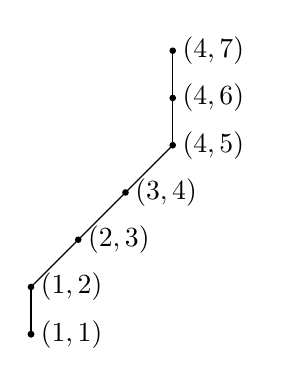
\begin{tikzpicture}[scale=0.6]

    % Start point
    \coordinate (A) at (1,1);
    % First step (0,1)
    \coordinate (B) at (1,2);
    % Second step (1,1)
    \coordinate (C) at (2,3);
    % Third step (1,1)
    \coordinate (D) at (3,4);
    % Fourth step (1,1)
    \coordinate (E) at (4,5);
    % Fifth step (1,1)
    \coordinate (F) at (4,6);
    % Final point
    \coordinate (G) at (4,7);

    % Draw the path
    \fill (1,1) circle (2pt) node[right] {$(1,1)$};
    \draw[-] (A) -- (B) node[right] {$(1,2)$};
    \draw[-] (B) -- (C) node[right] {$(2,3)$};
    \draw[-] (C) -- (D) node[right] {$(3,4)$};
    \draw[-] (D) -- (E) node[right] {$(4,5)$};
    \draw[-] (E) -- (F) node[right] {$(4,6)$};
    \draw[-] (F) -- (G) node[right] {$(4,7)$};

    % Draw the vertices
    \foreach \p in {A,B,C,D,E,F,G} {
        \fill[black] (\p) circle (2pt);
    }
\end{tikzpicture}
\end{center}

Since most of the paths in this paper will start from the point $(1,1)$, we will write $\lp_{A}$ instead of $\lp_{(1,1)\rightarrow A}$.

We shall assign weights to the step of the lattice path. For a north step $N$ that starts at $(k,n-1)$ and ends at $(k,n)$, we assign the weight $c(n,k)$. For the cross step $C$ that starts at $(k-1,n-1)$ and ends at $(k,n)$, we assign the weight $d(n,k)$. 

\begin{center}
    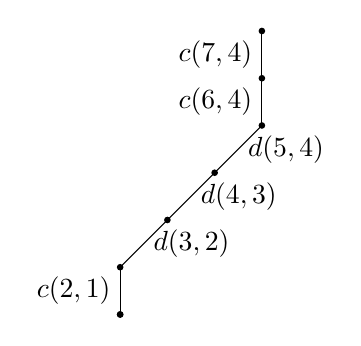
\begin{tikzpicture}[scale=0.6]

    % Start point
    \coordinate (A) at (1,1);
    % First step (0,1)
    \coordinate (B) at (1,2);
    % Second step (1,1)
    \coordinate (C) at (2,3);
    % Third step (1,1)
    \coordinate (D) at (3,4);
    % Fourth step (1,1)
    \coordinate (E) at (4,5);
    % Fifth step (1,1)
    \coordinate (F) at (4,6);
    % Final point
    \coordinate (G) at (4,7);

    % Draw the path
    \fill (1,1) circle (2pt);
    \draw[-] (A) -- (B) node[midway, left] {$c(2,1)$};
    \draw[-] (B) -- (C) node[midway, below, right] {$d(3,2)$};
    \draw[-] (C) -- (D) node[midway, below, right] {$d(4,3)$};
    \draw[-] (D) -- (E) node[midway, below, right] {$d(5,4)$};
    \draw[-] (E) -- (F) node[midway, left] {$c(6,4)$};
    \draw[-] (F) -- (G) node[midway, left] {$c(7,4)$};

    % Draw the vertices
    \foreach \p in {A,B,C,D,E,F,G} {
        \fill[black] (\p) circle (2pt);
    }
\end{tikzpicture}
\end{center}

The weight of a path $p \in \lp_{A \rightarrow B}$ is the product of the weights of the steps that make up the path. In our running example, it would be $c(2,1)d(3,2)d(4,3)d(5,4)c(6,4)c(7,4)$.
\begin{comment}

\end{comment}
\section{A log-concavity criterion for triangular arrays}
\subsection{Triangular arrays}
We have the following interpretation of a triangular array in terms of weighted lattice paths:
\begin{theorem}
    For $n\ge 1$ and $0<k \le n$, let $T(n,k)$ satisfy the following triangular recurrence.
    \begin{equation*}
        T(n,k)=c(n,k)\ T(n-1,k)+d(n,k)\ T(n-1,k-1).
    \end{equation*}
Then,
    \begin{equation*}
        T(n,k)=\displaystyle \sum_{p \in \lp_{(k,n)}} \wt(p).
    \end{equation*}
\end{theorem}
\begin{proof}
    We prove by induction on $n$. Each path in $\lp_{(k,n)}$ is either path in $\lp_{(k,n-1)}$ followed by an $N$ step or a path in $\lp_{(k-1,n-1)}$ followed by a cross step $C$. Since the weight of a path is the product of weight of the constituting steps, the statement follows from the recurrence.
    \end{proof}

Under this interpretation, we have the following interpretation of the log-concavity of rows.
\begin{corollary}
    The rows of the triangular array $T(n,k)$ are log-concave if and only if
\begin{equation*}
    \displaystyle \sum_{(p,q)\in \lp_{(k+1,n)}\times \lp_{(k-1,n)}} \wt(p)\wt(q) \le \displaystyle \sum_{(p',q')\in \lp_{(k,n)}\times \lp_{(k,n)}} \wt(p')\wt(q')
\end{equation*}
\end{corollary}
\begin{proof}
    The inequality $T(n,k)^2\ge T(n,k-1)T(n,k+1)$ is equivalent to \begin{equation*}
    \bigg(\displaystyle \sum_{p \in \lp_{(k,n)}} \wt(p)\bigg)^2 \ge \bigg( \displaystyle \sum_{p\in \lp_{(k-1,n)}} \wt(p)\bigg) \bigg(\displaystyle \sum_{q\in \lp_{(k+1,n)}} \wt(q)\bigg)
\end{equation*}
This can be written as 
\begin{equation*}
    \displaystyle \sum_{(p',q')\in \lp_{(k,n)}\times \lp_{(k,n)}} \wt(p')\wt(q') \ge \displaystyle \sum_{(p,q)\in \lp_{(k+1,n)}\times \lp_{(k-1,n)}} \wt(p)\wt(q). 
\end{equation*}
This completes our proof.
\end{proof}
\subsection{An injection from $\lp_{(k+1,n)}\times \lp_{(k-1,n)}$ to $\lp_{(k,n)}\times \lp_{(k,n)}$}
We shall describe an injective map that sends a pair of paths $(p,q)\in \lp_{(k+1,n)}\times \lp_{(k-1,n)}$ to a pair of paths $(p',q')\in \lp_{(k,n)}\times \lp_{(k,n)}$. The injection is based on an idea of Sagan \cite{sagan-log-concave} that is used to give injective proofs of log-concavity of the Stirling numbers of first and second kind. 

\begin{theorem}[Discrete Intermediate Value Theorem]\label{prop: DIVT}
Let $f$ be an integer-valued function on the integers in the interval $[m,n]$. Suppose that $|f(i+1)-f(i)|\le 1$ for $m\le i\le n$. If $f(m)f(n)<0$, then $f(x)=0$ for some integer $x \in [m,n]$.    
\end{theorem}

\begin{proposition}
    Let $(p,q)\in \lp_{(k+1,n)}\times \lp_{(k-1,n)}$ with $p=p_1\dots p_{n-1}$ and $q=q_1\dots q_{n-1}$. There is an index $1\le i\le n-1$ such that $p'=p_1\dots p_i q_{i+1}\dots q_{n-1}$ and $q'=q_1\dots q_i p_{i+1}\dots p_{n-1}$ are in $\lp_{(k,n)}\times \lp_{(k,n)}$.
\end{proposition}
\begin{proof}
Let $N:[0,n-1] \rightarrow \mathbb Z$ be the function defined by $N(0)=-1$ and $N(i)=\#\{ r\in [i]\ |\  p_r=C\} - \#\{ r \in [i]\ |\  q_r=C \}-1$ for $1\le i\le n-1$. Here, $|N(i+1)-N(i)|=1$ if either $p_{i+1}=C$ but $q_{i+1}\neq C$, or $p_{i+1}\neq C$ but $q_{i+1}=C$, and $|N(i+1)-N(i)|=0$ otherwise. Also, $N(0)=-1$ and $N(n-1)=1$ making $N(0)N(n-1)=-1<0$. Therefore, by Theorem \ref{prop: DIVT}, we have that $N(x)=0$ for some $x\in [n-1]$. Since $N(n-1)-N(x)=1$, we have that there is one more $C$ step in the remaining subword of $p$ than there is for $q$. Therefore, switching the subwords will have the intended effect.
\end{proof}
We are ready to define an injection $I$ from $\lp_{(k+1,n)}\times \lp_{(k-1,n)}$ to $\lp_{(k,n)}\times \lp_{(k,n)}$.
Given $(p,q) \in \lp_{(k+1,n)}\times \lp_{(k-1,n)}$ with $p=p_1\dots p_{n-1}$ and $q=q_1\dots q_{n-1}$, choose the largest index $i$ such that $p'=p_1\dots p_i q_{i+1}\dots q_{n-1}$ and $q'=q_1\dots q_i p_{i+1}\dots p_{n-1}$ belongs to $\lp_{(k,n)}\times \lp_{(k,n)}$. Then $I(p,q):=(p',q')$. The map is well-defined because of the previous proposition.

\begin{remark}\label{rem: imp}
    A step in path $q\in \lp_{k-1,n}$ after the index $i$ is moved exactly $1$ step to the right and a step that started at $(k_1,n_1)$ would now start at $(k_1+1,n_1)$ in the path $q'\in \lp_{(k,n)}$. Similarly, any step in path $p\in \lp_{k+1,n}$ would move exactly $1$ step to the left after the  index $i$. Any step that started at $(k_2,n_1)$ would now start at $(k_2-1,n_1)$ in the path $p'\in \lp_{(k,n)}$.
\end{remark}

\begin{example}
    Take the two paths $NNCNNN\in \lp_{(2,7)}$ and $NCCCNN\in \lp_{(4,7)}$. Under the injection, it would go to $NNCCNN$ and $NCCNNN$ in $\lp_{(3,7)}$. The index $i$ where the shift occurs is $3$.
\begin{center}
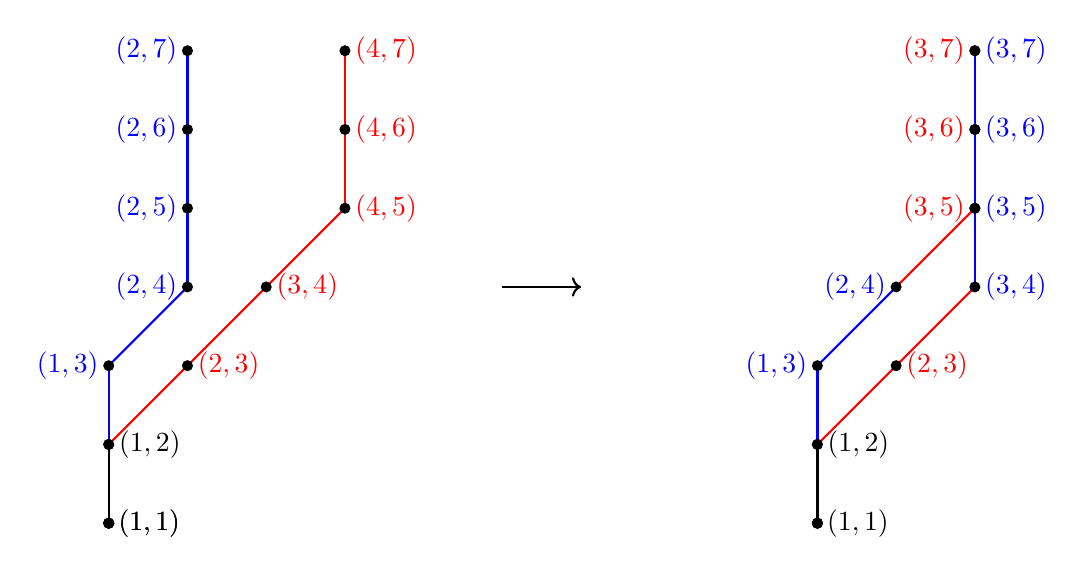
\begin{tikzpicture}[scale=1]
    % Draw the grid
    % \draw[very thin, gray] (0,0) grid (3,8);
    % Start point
    \coordinate (A) at (1,1);
    % First step (0,1)
    \coordinate (B) at (1,2);
    % Second step (1,1)
    \coordinate (C) at (1,3);
    % Third step (1,1)
    \coordinate (D) at (2,4);
    % Fourth step (1,1)
    \coordinate (E) at (2,5);
    % Fifth step (1,1)
    \coordinate (F) at (2,6);
    % Final point
    \coordinate (G) at (2,7);
    
    % Draw the points and the path
    \draw[-, thick, blue] (1,1) -- (1,2) ;
    \draw[-, thick, blue] (1,2) -- (1,3) node[left] {$(1,3)$};
    \draw[-, thick, blue] (1,3) -- (2,4) node[left] {$(2,4)$};
    \draw[-, thick, blue] (2,4) -- (2,5) node[left] {$(2,5)$};
    \draw[-, thick, blue] (2,5) -- (2,6) node[left] {$(2,6)$};
    \draw[-, thick, blue] (2,6) -- (2,7) node[left] {$(2,7)$};

    % Mark the starting and ending points
    \foreach \p in {A,B,C,D,E,F,G} {
        \fill[black] (\p) circle (2pt);
    }

    \coordinate (A) at (1,1);
    % First step (0,1)
    \coordinate (U) at (1,2);
    % Second step (1,1)
    \coordinate (V) at (2,3);
    % Third step (1,1)
    \coordinate (W) at (3,4);
    % Fourth step (1,1)
    \coordinate (X) at (4,5);
    % Fifth step (1,1)
    \coordinate (Y) at (4,6);
    % Final point
    \coordinate (Z) at (4,7);

    % Draw the path
    \fill (1,1) circle (2pt) node[right] {$(1,1)$};
    \draw[-, thick] (A) -- (U) node[right,black] {$(1,2)$};
    \draw[-, thick, red] (U) -- (V) node[right] {$(2,3)$};
    \draw[-, thick, red] (V) -- (W) node[right] {$(3,4)$};
    \draw[-, thick, red] (W) -- (X) node[right] {$(4,5)$};
    \draw[-, thick, red] (X) -- (Y) node[right] {$(4,6)$};
    \draw[-, thick, red] (Y) -- (Z) node[right] {$(4,7)$};

    % Draw the vertices
    \foreach \p in {A,U,V,W,X,Y,Z} {
        \fill[black] (\p) circle (2pt);
    }


   \draw[->,thick] (6,4)--(7,4);
    
\coordinate (a) at (10,1);
    % First step (0,1)
    \coordinate (b) at (10,2);
    % Second step (1,1)
    \coordinate (c) at (10,3);
    % Third step (1,1)
    \coordinate (d) at (11,4);
    % Fourth step (1,1)
    \coordinate (e) at (12,5);
    % Fifth step (1,1)
    \coordinate (f) at (12,6);
    % Final point
    \coordinate (g) at (12,7);
    
    % Draw the points and the path
    \fill (10,1) circle (2pt) node[right] {$(1,1)$};
    \draw[-, thick, blue] (10,1) -- (10,2);
    \draw[-, thick, blue] (10,2) -- (10,3) node[left] {$(1,3)$};
    \draw[-, thick, blue] (10,3) -- (11,4) node[left] {$(2,4)$};
    \draw[-, thick, red] (11,4) -- (12,5) node[left] {$(3,5)$};
    \draw[-, thick, red] (12,5) -- (12,6) node[left] {$(3,6)$};
    \draw[-, thick, red] (12,6) -- (12,7) node[left] {$(3,7)$};

    % Mark the starting and ending points
    \foreach \p in {a,b,c,d,e,f,g} {
        \fill[black] (\p) circle (2pt);
    }
\coordinate (a) at (10,1);
    % First step (0,1)
    \coordinate (u) at (10,2);
    % Second step (1,1)
    \coordinate (v) at (11,3);
    % Third step (1,1)
    \coordinate (w) at (12,4);
    % Fourth step (1,1)
    \coordinate (x) at (12,5);
    % Fifth step (1,1)
    \coordinate (y) at (12,6);
    % Final point
    \coordinate (z) at (12,7);

    % Draw the path
    \fill (1,1) circle (2pt) node[right] {$(1,1)$};
    \draw[-, thick] (a) -- (u) node[right,black] {$(1,2)$};
    \draw[-, thick, red] (u) -- (v) node[right] {$(2,3)$};
    \draw[-, thick, red] (v) -- (w) node[right,blue] {$(3,4)$};
    \draw[-, thick, blue] (w) -- (x) node[right,blue] {$(3,5)$};
    \draw[-, thick, blue] (x) -- (y) node[right,blue] {$(3,6)$};
    \draw[-, thick, blue] (y) -- (z) node[right,blue] {$(3,7)$};

    % Draw the vertices
    \foreach \p in {a,u,v,w,x,y,z} {
        \fill[black] (\p) circle (2pt);
    }
\end{tikzpicture}
\end{center}
\end{example}

In the next section, we give sufficient conditions for ensuring that $\wt(p,q) \le \wt I(p,q)$ for $(p,q)\in \lp_{(k+1,n)}\times \lp_{(k-1,n)}$.

\subsection{Proofs of Theorems \ref{thm: main} and \ref{thm: a,b,c}}

Usually, a $2$-Motzkin path of length $n$ is a lattice path starting from $(0,0)$ and $(n,0)$ that uses an up step $U:=(1,1)$, a down step $D:=(1,-1)$, a blue horizontal step $H_1:=(1,0)$ and a red horizontal $H_2:=(1,0)$. However, we will use the name $2$-Motzkin path to mean a lattice path with the steps described above but starting from $(0,0)$ and ending in $(n,-1)$ such that the last step is a down step $D$ and except for the last step, the remaining lattice path lies entirely above the $x$-axis.

To obtain a sufficient condition for log-concavity, we will associate a weighted $2$-Motzkin path to the pair of paths in $\lp_{(k+1,n)}\times \lp_{(k-1,n)}$ and use the weighted $2$-Motzkin path to create a sufficient condition that ensures the weight of pair of paths increases under the injection defined in the previous subsection. Let $(p,q)\in \lp_{(k+1,n)}\times \lp_{(k-1,n)}$. Let $\ch(p):=p_{i+1}\dots p_{n-1}$ and $\ch(q):=q_{i+1}\dots q_{n-1}$ where $i$ is largest index such that $p_1\dots p_i \ch(q)$ and $q_1\dots q_i \ch(p)$ are in $\lp_{(k,n)}$. 

The idea will be that the pair of paths $p,q$, when looked at from the end, start out with a spacing of $2$ ($(k-1,n)$ and $(k+1,n)$), continue with a spacing greater than or equal to $2$ and finally, getting down to a spacing of $1$ at the index $i$ prescribed by the injection. We will encode this portion of the paths as a $2$-Motzkin path.

To this end, consider the reversal operator $\rev$ on words. We start with the two words $\rev(\ch(p))$ and $\rev(\ch(q))$. We build a weighted $2$-Motzkin path out of the two words as follows. If the $j^{th}$ steps of $\rev(\ch(p))$ and $\rev(\ch(q))$ are $N$ and $C$ respectively (resp. $C$ and $N$ or $N$ and $N$ or $C$ and $C$), the $j^{th}$ step of our weighted $2$-Motzkin path is $U$ (resp. $D,H_1,H_2$). The weight of the step in the $2$-Motzkin path will be the product of the weight of the corresponding steps in $p$ and $q$. 

The fact that such a construction yields a weighted $2$-Motzkin path follows the fact that $i$ is the largest index such that $\ch(p)$ has one more $C$ step than $\ch(q)$. The $2$-Motzkin path will start at $(0,0)$ and end at $(n-i,-1)$. Except for the last $D$ step, the entire path will be above the $x$-axis. 
% {\color{blue}{(Just two more comments. For the same reason as the ordered pair confusion, the definition of weight of a step in the 2-Motzkin path was a little confusing to me initially. There should be a better way to phrase it... Also, just to be sure, is it not a part of the usual definition of a 2-Motzkin path that it lies completely above the x-axis? If so, maybe it's another reason to define 2-Motzkin paths initially, and say that you wish to permit them to go below the x-axis.)}}

The $2$-Motzkin path corresponding to our pair of paths is below. The blue steps correspond to $H_1$ steps.
\begin{center}
    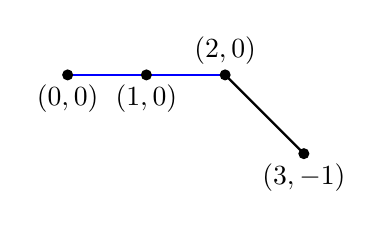
\begin{tikzpicture}[scale=1]
    \coordinate (A) at (0,0);
    \coordinate (B) at (1,0);
    \coordinate (C) at (2,0);
    \coordinate (D) at (3,-1);
 \draw[-,thick, blue] node[below, black] {$(0,0)$} (A)--(B) node[below,black] {$(1,0)$} ;
\draw[-,thick, blue]  (B)--(C) node[above, black] {$(2,0)$} ;
\draw[-,thick] (C)--(D)  node[below,black] {$(3,-1)$};

\foreach \p in {A,B,C,D} {
        \fill[black] (\p) circle (2pt);
    }
\end{tikzpicture}
\end{center}

Let us calculate the weight of the four different steps. The weight of $U$ step is $c(n_1,k_1)d(n_1,k_2)$, and the $D$ step is $d(n_1,k_1)c(n_1,k_2)$. The weight of a $H_1$ step is $c(n_1,k_1)c(n_1,k_2)$. The weight of a $H_2$ step is $d(n_1,k_1)d(n_1,k_2)$.

 On a $2$-Motzkin path, for each $U$ step, there is a corresponding $D$ step. That is if $(n_2,l_2)\in p$ and $(n_2,l_1)\in q$, there is a $(n_1,k_2)\in p$ and $(n_1,k_1)\in q$ such that the following are true.
 \begin{itemize}
     \item $n_2>n_1$, $l_2>k_2>k_1$, $l_2>l_1>k_1$,
     \item $k_2-k_1=l_2-l_1+1$,
     \item $n_2-n_1\ge l_2-k_2$ and $n_2-n_1\ge l_1-k_1$.
 \end{itemize}

We are in a position to prove Theorem \ref{thm: main}.
%  \begin{theorem}\label{thm: main}
%      For $n\ge 1$ and $0<k \le n$, let $T(n,k)$ satisfy the following triangular recurrence.
%     \begin{equation*}
%         T(n,k)=c(n,k)\ T(n-1,k)+d(n,k)\ T(n-1,k-1)
%     \end{equation*}
%     The sequence $(T(n,k))_{k=0}^n$ is log-concave if $(i),(ii)$ and $(iii)$ hold.
%     \begin{enumerate}
%         \item $c(n,k),d(n,k)$ are log-concave in $k$.
%         \item  Suppose \begin{itemize}
%      \item $n_2>n_1$; $l_2>k_2>k_1$; $l_2>l_1>k_1$,
%      \item $k_2-k_1=l_2-l_1+1$,
%      \item $n_2-n_1\ge l_2-k_2$ and $n_2-n_1\ge l_1-k_1$.
% \end{itemize} Then,
% $$c(n_1,k_1)d(n_1,k_2)d(n_2,l_1)c(n_2,l_2)\le c(n_1,k_1+1)d(n_1,k_2-1)d(n_2,l_1+1)c(n_2,l_2-1)$$ 
%         \item For all $k$, we have $d(n_1,k+1)c(n_1,k)\le d(n_1,k)c(n_1,k+1)$.
%     \end{enumerate}
%  \end{theorem}
\begin{proof}[Proof of Theorem \ref{thm: main}]
The weight of a $H_1$ step is $c(n_1,k_1)c(n_1,k_2)$ which goes, under the injection, to a $H_1$ step whose weight is $c(n_1,k_1+1)c(n_1,k_2-1)$ (see Remark \ref{rem: imp}). Similarly, for $H_2$, $d(n_1,k_1)d(n_1,k_2)$ goes to $d(n_1,k_1+1)d(n_1,k_2-1)$. Therefore, Condition $(i)$ ensures that $\wt(H_1)\le \wt(I(H_1))$ and $\wt(H_2)\le \wt(I(H_2))$.

Similarly, Condition $(ii)$ ensures that the product of the weights of a $U$ and its corresponding $D$ step in the path is greater after applying the injection. 

Finally, Condition $(iii)$ ensures that the final $D$ step is greater after applying the injection.

These three conditions ensure that 
\begin{equation*}
    \displaystyle \sum_{(p,q)\in \lp_{(k+1,n)}\times \lp_{(k-1,n)}} \wt(p)\wt(q) \le \displaystyle \sum_{(p',q')\in \lp_{(k,n)}\times \lp_{(k,n)}} \wt(p')\wt(q')
\end{equation*}
Therefore, the sequence $T(n,k)$ is log-concave in $k$.
\end{proof}

\begin{remark}
    It should be possible to weaken Condition $(iii)$ or completely remove it by sufficiently strengthening the other two conditions.
\end{remark}

The following is a quick application of this theorem. The Legendre-Stirling numbers were shown to be log-concave \cite{andrews-legendre-stirling}. It is easy to verify that the coefficients satisfy the above theorem, therefore, giving us another proof of their log-concavity.
\begin{corollary}
    The Legendre-Stirling numbers defined by
    \begin{equation}
        LS(n,k)=(k^2+k)LS(n-1,k)+LS(n-1,k-1)
    \end{equation}
    are log-concave in $k$ for all $n$.
\end{corollary}

% \begin{corollary}\label{cor: d=1}
%     For $n\ge 1$ and $0\le k \le n$, let $T(n,k)$ satisfy the following triangular recurrence.
%     \begin{equation*}
%         T(n,k)=c(n,k)T(n-1,k)+T(n-1,k-1)
%     \end{equation*}
%     The sequence $(T(n,k))_{k=0}^n$ is log-concave if 
%     \begin{enumerate}
%         \item $c(n,k)$ is log-concave in $k$.
%         \item $c(n_1,k_1)c(n_2,l_1)\le c(n_1,k_1+1)c(n_2,l_1-1)$ for $n_2>n_1$, $l_1>k_1$ and $n_2+k_1\ge n_1+l_1$.
%         \item $c(n,k)$ is increasing in $k$.
%         \end{enumerate}
% \end{corollary}
The following is an observation that follows from the form of the conditions in Theorem \ref{thm: main}.
\begin{corollary}\label{cor: multiplicative}
    For $c(n,k),d(n,k)\ge 0$, if the triangular array $$T(n,k)=c(n,k)T(n-1,k)+d(n,k)T(n-1,k-1)$$ satisfies the conditions of Theorem \ref{thm: main}, then for $l\in \mathbb{N}$, so does the array $$\widetilde{T}(n,k)=c(n,k)^l\widetilde{T}(n-1,k)+d(n,k)^l\widetilde{T}(n-1,k-1).$$ 
\end{corollary}
Using the two aforementioned results, we can prove the main result of the paper.
% \begin{theorem}\label{thm: a,b,c}
%     Let $\alpha,\beta,\gamma$ and $\alpha',\beta',\gamma'$ be real numbers such that the following hold:
%     \begin{enumerate}
%         \item $\alpha, \alpha',\beta\ge 0$
%         \item $\beta'\in [-\alpha',0]$
%         \item $\alpha+\beta+\gamma,\ \alpha'+\beta'+\gamma'\ge 0$
%     \end{enumerate}
%     Then \begin{equation}
%         T(n,k)=(\alpha n+\beta k+\gamma)^l\ T(n-1,k)+(\alpha'n+\beta'k+\gamma')^l \ T(n-1,k-1)
%     \end{equation}
%     is log-concave in $k$ for all $n$.
% \end{theorem}
\begin{proof}[Proof of Theorem \ref{thm: a,b,c}]
    Condition (i) is easily verified.
    We insist that $\alpha, \alpha'\ge 0$. Otherwise, for all large $n$, we would have $\alpha n +\beta k+\gamma$ or $\alpha'n+\beta' k+\gamma'$ becoming negative. Similarly, we insist on $\alpha+\beta+\gamma, \alpha'+\beta'+\gamma'\ge 0$ for ensuring the non-negativity of $c(n,k),d(n,k)$. We want to show that conditions $(ii), (iii)$ of Theorem \ref{thm: a,b,c} are enough to apply Theorem \ref{thm: main}. 
    
    $\textbf{Verifying Condition (ii):}$ 
    \begin{eqnarray*}
         &&c(n_1,k_1+1)c(n_2,l_2-1)-c(n_1,k_1)c(n_2,l_2)\\
         &=& (\alpha n_1 +\beta k_1+\gamma+\beta)(\alpha n_2+\beta l_2+\gamma-\beta)-(\alpha n_2+\beta k_1+\gamma)(\alpha n_2+\beta l_2+\gamma)\\
         &=& \alpha\beta (n_2-n_1)+\beta^2(l_2-k_1-1) \ge 0
\\
\\
       &&d(n_1,k_2-1)d(n_2,l_1+1)-d(n_1,k_2)d(n_2,l_1)\\
        &=&(\alpha' n_1+\beta' k_2+\gamma'-\beta')(\alpha'n_2+\beta'l_1+\gamma'+\beta')-(\alpha'n_1+\beta'k_2+\gamma')(\alpha'n_2+\beta'l_1+\gamma')\\
        &=& -\beta' ( \alpha'(n_2-n_1)+ \beta'(l_1-k_2+1)) \ge 0
    \end{eqnarray*}
    The last line follows because $\alpha'(n_2-n_1)\ge\alpha'(l_1-k_1)\ge\alpha'(l_1-k_2+1)\ge|\beta'|(l_1-k_2+1)$ and so, $ \alpha'(n_2-n_1)+ \beta'(l_1-k_2+1)\ge 0$.

    $\textbf{Verifying Condition (iii):}$  
    \begin{eqnarray*}
     &&\frac{d(n_1,k+1)}{d(n_1,k)}\frac{c(n_1,k)}{c(n_1,k+1)}\le 1\\
    \end{eqnarray*}
    Since $\beta'\le 0$, $d(n,k)$ increases as $k$ decreases and since $\beta\ge0$, $c(n,k)$ increases as $k$ increases.
\end{proof}
\begin{remark}
    The conditions $\alpha+\beta+\gamma\ge 0$ and $\alpha'+\beta'+\gamma'\ge 0$ exist to ensure that coefficients $c,d$ are non-negative. One may increase $\gamma,\gamma'$ by non-negative integers and retain log-concavity of the sequence.
\end{remark}

\begin{corollary}
    The $(l,r)$-Lah numbers are log-concave in $k$ for all $n$.
\end{corollary}
\begin{proof}
    The $(l,r)$-Lah numbers satisfy the recurrence relation
    \begin{equation}
        T(n,k)=(n+k+2r-3)^l\ T(n-1,k)+T(n-1,k-1)
    \end{equation}
    with the initial condition $T(0,0)=1$. By Theorem \ref{thm: a,b,c}, we have that this triangular array is log-concave in $k$ for all $n$.
\end{proof}
% Given below is a table of well known sequences in the literature that satisfy the hypotheses of Theorem \ref{thm: a,b,c}.
% \begin{table}[ht]
% \centering
% \begin{tabular}{|l|l|l|}
% \hline
% \textbf{Parameters $(\alpha,\beta,\gamma;\  \alpha',\beta',\gamma')$} & \textbf{Name ($l=1$) and Reference} & \textbf{OEIS Entry} \\
% \hline
% % Add your data rows below
% $(0,1,1;\nu,-1,1-\nu)$ & $\nu$-order Eulerian numbers \cite{higher-order-eulerian} & A173018, A008517, A219512 \\
% $(0,j,1;\ j,-j,0)$ & $1/j$-Eulerian numbers \cite{1/k-eulerian} & \\
% $(0,1,0;\ 0,0,1)$ & Stirling subset numbers & A008277\\
% $(1,1,-1;\ 0,0,1)$ & Lah numbers & A015278\\
% $(1,m,-1;\ 0,0,m)$ & $m-$associated Lah numbers&\\
% $(2,1,-2;\ 0,0,1)$ & Generalisation of Lah, Stirling numbers  \cite{stirling-lah} & A035342\\
% $(r-1,1,1-r;\ 0,0,1)$ & $S(r,n,k)$ \cite{broder-r-stir}& \\
% $(0,0,1;\ 0,0,1)$ & Binomial Coefficients & A007318\\
% $(1,0,-1;\ 0,0,1)$ & Stirling cycle numbers & A132393\\
% $(1,2,-1;\ 3,-2,1)$ & Scaled type A Narayana numbers \cite{ma-gamma-descent} & \\
% $(1,2,0;\ 3,-2,0)$ & Scaled type B Narayana numbers \cite{ma-gamma-descent}& \\
% $(2,1,-1;\ 0,0,1)$ & Holiday numbers of first kind \cite{Szekely-holiday}&\\
% $(2,1,0;\ 0,0,1)$& Holiday numbers of second kind \cite{Szekely-holiday}& \\
% \hline
% \end{tabular}
% \caption{Some sequences of combinatorial interest satisfying Theorem \ref{thm: a,b,c}.}
% \label{tab:parameters}
% \end{table}
\begin{comment}
In the next subsection, we give multiple applications of these terms to show log-concavity of commonly encountered triangular arrays.
\subsection{Applications}
\begin{enumerate}
    \item The Eulerian numbers
    $$T(n,k)=(k+1)T(n-1,k)+(n-k)T(n-1,k-1).$$
\begin{proof}
    Clearly, $k+1$ and $n-k$ are log-concave. Now, $$c(n_1,k_1)d(n_1,k_2)d(n_2,l_1)c(n_2,l_2)=(k_1+1)(n_1-k_2)(n_2-l_1)(l_2+1)$$
    and $$c(n_1,k_1+1)d(n_1,k_2-1)d(n_2,l_1+1)c(n_2,l_2-1)=(k_1+2)(n_1-k_2+1)(n_2-l_1-1)l_2$$
    From the hypothesis of condition $(ii)$, we have $l_2+1>k_1+1$ as $l_2>k_1$. Similarly, $n_2-l_1 \ge n_1-k_1 > n_1-k_2$ from the hypothesis of condition $(ii)$. Therefore, inequality in condition $(ii)$ is satisfied.
    Condition $(iii)$ is satisfied as $c(n,k)$ increases as $k$ increases and $d(n,k)$ decreases as $k$ increases.
\end{proof}
    \item The $1/j$-Eulerian numbers
    $$T(n,k)=(jk+1)T(n-1,k)+j(n-k)T(n-1,k-1).$$
\begin{proof}
Once again, $jk+1$ and $j(n-k)$ are concave. Now, $$c(n_1,k_1)d(n_1,k_2)d(n_2,l_1)c(n_2,l_2)=(jk_1+1)j(n_1-k_2)j(n_2-l_1)(jl_2+1)$$
    and $$c(n_1,k_1+1)d(n_1,k_2-1)d(n_2,l_1+1)c(n_2,l_2-1)=(jk_1+2)j(n_1-k_2+1)j(n_2-l_1-1)jl_2$$   
    From the previous proof, we can verify condition $(ii)$. Condition $(iii)$ is satisfied as $c(n,k)$ increases as $k$ increases and $d(n,k)$ decreases as $k$ increases.
\end{proof}
\item The Stirling number of second kind.
$$T(n,k)=kT(n-1,k)+T(n-1,k-1).$$
We show these numbers are log-concave by appealing to Theorem \ref{cor: d=1}. The sequence $k$ is log-concave in $k$. We have $k_1l_1\le (k_1+1)(l_1-1)$, which satisfies condition $(ii)$ of Theorem \ref{cor: d=1}. Clearly, $k$ increases with $k$.
\item The Stirling number of first kind.
$$T(n,k)=(n-1)T(n-1,k)+T(n-1,k-1)$$
Clearly, all three conditions of Theorem \ref{cor: d=1} are satified.
\item The Lah number.
$$T(n,k)=(n+k-1)T(n-1,k)+T(n-1,k-1).$$
We can verify the conditions of Theorem \ref{cor: d=1}. Clearly, $n+k-1$ is log-concave in $k$ and is increasing in $k$. This verifies conditions $(i)$ and $(iii)$. Now, 
$$c(n_1,k_1)c(n_2,l_1)= (n_1+k_1-1)(n_2+l_1-1)$$
and $$c(n_2,l_1-1)c(n_1,k_1+1)=(n_2+l_1-2)(n_1+k_1).$$
Since $n_2>n_1$ and $l_1> k_1$, we have $n_2+l_1>n_1+k_1$ and so, $$(n_2+l_1-2)(n_1+k_1)\ge (n_2+l_1-1)(n_1+k_1-1),$$ which is condition $(ii)$.

The next four follow from Theorem $\ref{cor: multiplicative}$.
    \item The generalised $(l,r)$-Stirling number of second kind.
$$T(n,k)=(k+r-1)^lT(n-1,k)+T(n-1,k-1).$$
% Here, $d(n,k)=1$ and $c(n,k)=k$.
% We have $k_1l_1\le (k_1+1)(l_1-1)$, which is true.
\item The generalised $(l,r)$-Stirling number of first kind.
$$T(n,k)=(n+r-2)^lT(n-1,k)+T(n-1,k-1)$$
\item The generalised $(l,r)$-Lah number.\cite[Conjecture 9]{aleks-gen-lah}
$$T(n,k)=(n+k+2r-3)^lT(n-1,k)+T(n-1,k-1).$$
\item The generalised $(l,r)$- Eulerian number.
$$\eul^{(l)}_r(n,k)=(n-k)^l\eul^{(l)}_r(n-1,k-1)+(k+r)^l\eul^{(l)}_r(n-1,k)$$
\end{enumerate}


\end{comment}
\section{Two parameter generalization of Eulerian numbers}\label{sec: 2-para }

Recall that we defined $\eul_r^{(l)}(n,k)$ to count the number of $l$-tuples $(f_1,\dots, f_l)$ such that $[r]\subset \bl(f_1)$, $|\bl(f_1)|=k+1$, and $\bl(f_1)=\dots=\bl(f_l)$. We first start out by proving a recurrence relation for the $(l,r)$-Eulerian numbers. They satisfy a triangular recurrence analogous to the ones satisfied by their Stirling and Lah counterparts.
\begin{proposition}
    For $n\ge k\ge r-1\ge0$ and a positive integer $l$, we have 
    \begin{equation}
        \eul_r^{(l)}(n,k)=(n-k)^l \eul_r^{(l)}(n-1,k-1)+(k+1)^l\eul_r^{(l)}(n-1,k)
    \end{equation}
    and $\eul_r^{(l)}(r,r)=1$
\end{proposition}
\begin{proof}
     Let $f$ be a subexceedant function with $k+1$ elements in $\bl(f)$ and $[r]\subset \bl(f)$. Then, $f$ could have been obtained in one of the following two ways.
    \begin{enumerate}
        \item if $n\in \bl(f_i)$, its image has one of $(n-k)^l$ choices,
        \item if not, then its image has one of $(k+1)^l$ choices.
    \end{enumerate}
\end{proof}

\begin{remark}
      By Theorem \ref{thm: a,b,c}, the $(l,r)$-Eulerian numbers are log-concave and therefore, unimodal.    
\end{remark}

\subsection{A bijection}
Let $\pi\in \SSS_n$. 
Define the block leaders of $\pi$, denoted by $\bl(\pi)$, as the set of first letters of the increasing runs of $\pi$. For example, let $\pi=28|7|4|136|5$ with bars separating increasing runs. Then, $\bl(\pi)=\{ 1,2,4,5,7 \}$. 
We show that $\eul_r(n,k):=\eul^{(1)}_r(n,k)$ also counts the number of permutations $\pi\in \SSS_n$ with $k$ descents such that $[r]\subset \bl(\pi)$.

Starting from a subexceedant function $f$ that satisfies $[r]\subset \bl(f)$ and $|\bl(f)|=k+1$, we give a map $\Lambda$ to a permutation $\pi$ with $k$ descents such that $[r]\subset \bl(\pi)$ with the additional property that $f(\bl(f))=\bl(\pi)$.

We give the bijection $\Lambda$ inductively. Start with the empty word and $i=1$. If $f(i)=i$, add $i$ to the left of all existing letters. If $f(i)\in f([i-1])$, then add $i$ at the end of the increasing run starting at $f(i)$. If $f(i)\notin f([i-1])$, then add $i$ immediately to the left of element $f(i)$. Increase $i$ to $i+1$ and repeat.

\begin{example}
    Starting with the subexceedant function $f=12121547$, we show the steps.
    \begin{eqnarray*}
        \phi\rightarrow 1 \rightarrow 21\rightarrow 213\rightarrow 2413\rightarrow 24135\\
        \rightarrow 241365 \rightarrow 2741365\rightarrow 28741365
    \end{eqnarray*}
    Therefore, $\Lambda(12121547)=28741365$.
    Note that the $f(\bl(f))=\{ 1,2,4,5,7 \} =\bl(28741365)$.
\end{example}

We can reconstruct the subexceedant function given a permutation $\pi$ as follows. For $1\le i\le n$, let $\pi|_i$ be the permutation with all letters greater than $i$ removed. In our running example, $\pi|_5=24135$.
If $i$ appears to the left of all elements in $\pi|_{i}$, then $f(i)=i$. If $i$ appears in front of some element $j\notin f([i-1])$, then $f(i)=j$. Else, $f(i)$ is the closest element from $f([i-1])$ to the left of $i$. 
\begin{example}
    Start with $\pi=28741365$. Here, $\pi|_1=1$, $\pi|_2=21$, $\pi|_3=213$, $\pi|_4=2413$, $\pi|_5=24135$, $\pi|_6=241365$, $\pi|_{7}=2741365$ and $\pi|_8=28741365$. 
    It is easy to check that $f(1)=1,f(2)=2$. $f(3)=1$ because $1$ the closest element in $f([2])$ to the left of $3$. $f(4)=2$, $f(5)=1$, in the same way. $f(6)=5$ because $5\notin f([5])$. Similarly, $f(7)=4$ and $f(8)=7$.
\end{example}

\begin{proposition}
    The map $\Lambda$ from the set of subexceedant functions from $[n]$ to $[n]$ such that $[r]\in \bl(f)$, $|\bl(f)|=k+1$ to the set of permutations on $[n]$ such that $[r]\in \bl(\pi)$, $|\bl(\pi)|=k+1$ is a bijection such that $f(\bl(f))=\bl(\Lambda(f))$.
\end{proposition}
\begin{proof}
    It is clear that the function $\Lambda$ is a bijection as we are able to describe its inverse. It remains to show that $f(\bl(f))=\bl(\Lambda(f))$. Suppose $f(i)\notin f([i-1])$, then $i$ goes behind $f(i)$, making $f(i)$ the first element of an increasing run. Similarly, the elements $i$ such that $f(i)=i$ are added to the leftmost position and therefore, are first elements of an increasing run. Therefore, the block leaders of $\Lambda(f)$ are exactly the elements of $f(\bl(f))$.
\end{proof}
% \subsection{Recurrence and an identity}
% \begin{proposition}
%     For $n\ge k\ge r-1\ge 0$, we have 
%     \begin{equation}
%         \eul_r(n,k)=(n-k)\eul_r(n-1,k-1)+(k+1)\eul_r(n-1,k).
%     \end{equation}
% \end{proposition}
% \begin{proof}
%      Let $f$ be a subexceedant function with $k+1$ elements in $\bl(f)$ and $[r]\subset \bl(f)$. Then, $f$ could have been obtained in one of the following two ways.
%     \begin{enumerate}
%         \item if $n\in \bl(f)$, its image has one of $n-k$ choices,
%         \item if not, then its image has one of $k+1$ choices.
%     \end{enumerate}
% \end{proof}
We have the following connection between the $r$-Stirling number of the second kind and $\eul_r(n,k)$. When $r=1$, this identity specialises to B\'ona \cite[Theorem 1.18]{bona-combin-permut}.
\begin{theorem} For $n\ge k\ge r-1\ge 0$, we have
    \begin{equation}\label{r-stir-eul}
        k!S_r(n,k)=\sum_{i=r}^{k}\eul_r(n,i-1)\binom{n-i}{k-i}.
    \end{equation}
\end{theorem}
\begin{proof}
    The LHS is the number of ordered partitions $\Pi$ of $[n]$ into $k$ blocks such that $[r] \subset \bl(\Pi)$. We need to show that RHS counts the same objects. Let $\pi\in \SSS_n$ with $i-1$ descents and $[r]\subset \bl(\pi)$. The $i$ increasing runs of $\pi$ give us an ordered partition of $[n]$. Now, the number of blocks is $i$, which can be smaller than $k$. However, we can make more blocks by making splits of the increasing runs. We need to make $k-i$ splits. This can be done by choosing $k-i$ of the $n-i$ different places where we can split.

    We just need to now show that the ordered partitions thus formed are all distinct. However, given an ordered partition $\Pi$ of $[n]$, we can arrange the blocks in ascending order internally and read from left to right a unique permutation and the choice of splitting from which it can be obtained.
\end{proof}

\begin{corollary} For $n\ge k\ge r-1\ge 0$, we have
    \begin{equation}
        \eul_r(n,k-1)=\sum_{i=1}^{k}(-1)^{k-i}S_r(n,i)\binom{n-i}{k-i}i!
    \end{equation}
\end{corollary}
\begin{proof}
    Equation \ref{r-stir-eul} can be rewritten as $\sum_{k=r}^n\eul_r(n,k-1)(t+1)^k=\sum_{k=r}^nk!S_r(n,k)t^{n-k}$.
    The corollary follows from the substitution $t\rightarrow t-1$.
\end{proof}
\subsection{Palindromicity of the associated generalised Eulerian polynomials}
% In this section, let us restrict our attention to the case when $r=1$.

% Define \[ \eul_n^{(l)}(s,t):= \displaystyle \sum_{k=0}^{n-1} \eul^{(l)}(n,k)s^kt^{n-1-k}. \]
% Let $\dd_s=s\frac{\partial }{\partial s}$ and $\dd_t=t\frac{\partial }{\partial t}$ in $\mathbb Q[s,t]$.

% \begin{proposition}
%     The polynomials $\eul^{(l)}_n(s,t)$ satisfy the following partial differential equation.
%     \begin{equation}
%         \eul^{(l)}_n(s,t)= \frac{1}{s} \dd_s^l(st\eul^{(l)}_{n-1}(s,t))+ \frac{1}{t} \dd_t^l(st\eul^{(l)}_{n-1}(s,t))
%     \end{equation}
%     with $\eul^{(l)}_0(s,t)=1$ initially.
% \end{proposition}
% \begin{proof}
    
% \end{proof}
% Notice that $\dd_s,\dd_t$ are linear operators on $\mathbb{Q}[s,t]$. Indeed, we have 
% $\dd_s(af+bg)=s\frac{\partial (af+bg)}{\partial s}=as\frac{\partial f}{\partial s}+bs\frac{\partial g}{\partial s}=a\dd_s(f)+b\dd_s(g).$

% \begin{proposition}
%     The polynomials $\eul_n^{(2)}(s,t)$ satisfy the recurrence relation
%     \begin{equation}
%         \eul_n^{(2)}(s,t) = (s+t)\eul_{n-1}^{(2)}(s,t) + 3st(\frac{\partial }{\partial s}+\frac{\partial }{\partial t})\eul_{n-1}^{(2)}(s,t)+ st(s\frac{\partial^2 }{\partial s^2} + t\frac{\partial^2 }{\partial t^2})\eul_{n-1}^{(2)}(s,t)
%     \end{equation}
%     with $\eul_0^{(3)}(s,t)=1$ initially.
% \end{proposition}

% \begin{proposition}
%     The polynomials $\eul_n^{(3)}(s,t)$ satisfy the recurrence relation
%     \begin{equation}
%         \eul_n^{(3)}(s,t) = (\frac{\partial }{\partial s}+\frac{\partial }{\partial t})(st\eul_{n-1}^{(3)}(s,t)) + 3(s\frac{\partial^2 }{\partial s^2}+t\frac{\partial^2 }{\partial t^2})(st\eul_{n-1}^{(3)}(s,t))+ (s^2\frac{\partial^3 }{\partial s^3} + t^2\frac{\partial^3 }{\partial t^3})(st\eul_{n-1}^{(3)}(s,t))
%     \end{equation}
%     with $\eul_0^{(2)}(s,t)=1$ initially.
% \end{proposition}
In this section, let us restrict our attention to the case when $r=1$.
We define associated $(l,1)$-Eulerian polynomials to be
\begin{equation}
    \eul_n^{(l)}(t):=\sum_{k=0}^{n-1} \eul^{(l)}(n,k)t^k.
\end{equation}
It is not immediately clear that this polynomial is palindromic. To that end, we define \begin{equation}\label{eq: r=1 eul}
     \eul_n^{(l)}(s,t):= \displaystyle \sum_{k=0}^{n-1} \eul^{(l)}(n,k)s^kt^{n-1-k}.
\end{equation} 
We show that the polynomial $\eul_n^{(l)}(s,t)$ is symmetric in $s,t$, i.e.,
$\eul_n^{(l)}(s,t)=\eul_n^{(l)}(s,t)$. Let $\dd_s=s\frac{\partial }{\partial s}$ and $\dd_t=t\frac{\partial }{\partial t}$ in $\mathbb Q[s,t]$.
The symmetry becomes apparent from the following proposition.

\begin{proposition}\label{prop: diff-recurrence}
    The polynomials $\eul^{(l)}_n(s,t)$ satisfy the following partial differential equation.
    \begin{equation}
        \eul^{(l)}_n(s,t)= \frac{1}{s} \dd_s^l(st\eul^{(l)}_{n-1}(s,t))+ \frac{1}{t} \dd_t^l(st\eul^{(l)}_{n-1}(s,t))
    \end{equation}
    with $\eul^{(l)}_0(s,t)=1$ initially.
\end{proposition}
\begin{proof}
    \begin{eqnarray*}
        \dd_s^l(st\eul^{(l)}_{n}(s,t)) & = & t \dd_s^l(s\eul^{(l)}_{n}(s,t))\\
        & = & t\bigg( \dd_s^l(\sum_{k=0}^{n} \eul^{(l)}(n,k) s^{k+1} t^{n-1-k}) \bigg)\\ 
        & = & \sum_{k=0}^{n-1}(k+1)^l\eul^{(l)}(n,k) s^{k+1} t^{n-k}
    \end{eqnarray*}
    Similarly,
    \begin{eqnarray*}
        \dd_t^l(st\eul^{(l)}_{n}(s,t)) & = & s \dd_t^l(t\eul^{(l)}_{n}(s,t))\\
        & = & s\bigg( \dd_t^l(\sum_{k=0}^{n} \eul^{(l)}(n,k) s^{k} t^{n-k}) \bigg)\\ 
        & = & \sum_{k=0}^{n-1}(n-k)^l\eul^{(l)}(n,k) s^{k+1} t^{n-k}
    \end{eqnarray*}
    Therefore, the RHS of the proposition evaluates the polynomial
    \begin{equation*}
        \sum_{k=0}^{n-1}(k+1)^l\eul^{(l)}(n,k) s^{k} t^{n-k}+\sum_{k=0}^{n-1}(n-k)^l\eul^{(l)}(n,k) s^{k+1} t^{n-1-k}
    \end{equation*}
    Comparing coefficients with \eqref{eq: r=1 eul} gives us the result. 
\end{proof}
% We also give a bijective proof of this fact to better understand the structure of the objects in question.

A palindromic polynomial $p(x)=\displaystyle\sum_{k=0}^n a_nx^k$ is said to be gamma-positive of center of symmetry $\lfloor \frac{n}{2}\rfloor$ if it can be written in the form $p(x)=\displaystyle\sum_{i=0}^{\lfloor\frac{n}{2} \rfloor} \gamma_{n,i}t^i(1+t)^{n-2i}$.
In light of the palindromicity of these polynomials, it would be the next natural question to ask if they are gamma-positive. It is not
difficult to show that these polynomials are gamma-positive when $l=2$.
% Notice that $\dd_s,\dd_t$ are linear operators on $\mathbb{Q}[s,t]$. Indeed, we have 
% $\dd_s(af+bg)=s\frac{\partial (af+bg)}{\partial s}=as\frac{\partial f}{\partial s}+bs\frac{\partial g}{\partial s}=a\dd_s(f)+b\dd_s(g).$
The following is the recurrence \ref{prop: diff-recurrence} for the polynomials written out. 
\begin{proposition}
    The polynomials $\eul_n^{(2)}(s,t)$ satisfy the recurrence relation
    \begin{equation}
        \eul_n^{(2)}(s,t) = (s+t)\eul_{n-1}^{(2)}(s,t) + 3st(\frac{\partial }{\partial s}
        +\frac{\partial }{\partial t})\eul_{n-1}^{(2)}(s,t)+ st(s\frac{\partial^2 }{\partial s^2}
         + t\frac{\partial^2 }{\partial t^2})\eul_{n-1}^{(2)}(s,t)
    \end{equation}
    with $\eul_0^{(2)}(s,t)=1$ initially.
\end{proposition}
It is straightforward to show that $$s\frac{\partial^2 }{\partial s^2}
+ t\frac{\partial^2 }{\partial t^2}$$
sends an element of the gamma-basis $(st)^i(s+t)^{n-1-i}$ to a positive linear combination of gamma basis elements as do 
the other two terms. Since these are linear operators, we have that the polynomials are gamma-positive by induction. If we set $s=1$, we get

\begin{proposition}
    The polynomials $\eul_n^2(t):=\displaystyle \sum_{k=0}^{n-1} \eul^{(2)}(n,k)t^k$ are gamma-positive for all $n\ge 2$.
\end{proposition}

Here are the polynomials $\eul_n^3(t)$ and their expansion in the gamma-basis.
\begin{eqnarray*}
    \eul_3^3(t)&=& 1+16t+t^2=(1+t)^2+14t\\
    \eul_4^3(t)&=& 1+155t+155t^2+t^3=(1+t)^3+152t(1+t)\\
    \eul_5^3(t)&=& 1+1304t+8370t^2+1304t^3+t^4=(1+t)^4+1300t(1+t)^2+5764t^2\\
    \eul_6^3(t)&=& 1+10557t+309446t^2+309446t^3+10557t^4+t^5=(1+t)^5+10552t(1+t)^3+277780t^2(1+t)
\end{eqnarray*}

\begin{remark}
We know that the Eulerian polynomials are gamma-positive and we have proved that the $(2,1)$-Eulerian polynomials are gamma-positive.
    Based on the limited data that we were able to compute, the $(l,1)$-Eulerian polynomials seem to be gamma-positive for all $l\ge 3$.
\end{remark}

\begin{remark}
    A similar remark can be made about real-rootedness. The Eulerian polynomials are known to be real rooted due to Frobenius \cite{frobenius-real-root-eulerian}. From our limited data, it appears that the $(l,1)$-Eulerian polynomials are real rooted for $l\ge 2$. 
\end{remark}
% \begin{remark}
%     From limited data, it appears these polynomials might be gamma-positive and real-rooted for all $l\in \N$.
% \end{remark}
% \bibliography{thesis}
\begin{thebibliography}{10}

\bibitem{andrews-legendre-stirling}
{\sc Andrews, G.~E., Gawronski, W., and Littlejohn, L.~L.}
\newblock The {Legendre}-{Stirling} numbers.
\newblock {\em Discrete Math. 311}, 14 (2011), 1255--1272.

\bibitem{higher-order-eulerian}
{\sc Barbero~G., J.~F., Salas, J., and Villase{\~n}or, E. J.~S.}
\newblock Generalized {Stirling} permutations and forests: higher-order {Eulerian} and {Ward} numbers.
\newblock {\em Electron. J. Comb. 22}, 3 (2015), research paper p3.37, 20.

\bibitem{lr-stir-ref}
{\sc Belbachir, H., and Djemmada, Y.}
\newblock The $(l,r)$-{Stirling} numbers: a combinatorial approach.
\newblock Preprint, {arXiv}:2101.11039 [math.{CO}] (2021), 2021.

\bibitem{bona-combin-permut}
{\sc B{\'o}na, M.}
\newblock {\em Combinatorics of {P}ermutations}, 2nd~ed.
\newblock Chapman and Hill, CRC Press, 2012.

\bibitem{branden-unimodality_log_concavity}
{\sc Br{\"a}nd{\'e}n, P.}
\newblock Unimodality, {L}og-concavity, {R}eal-rootedness and {B}eyond.
\newblock In {\em Handbook of Enumerative Combinatorics}, M.~Bona, Ed. Chapman \& Hall \/ CRC Press, 2015, ch.~7.

\bibitem{broder-r-stir}
{\sc Broder, A.~Z.}
\newblock The {{\(r\)}}-{Stirling} numbers.
\newblock {\em Discrete Math. 49\/} (1984), 241--259.

\bibitem{frobenius-real-root-eulerian}
{\sc Frobenius, G.}
\newblock {\em {\"U}ber die Bernoullischen Zahlen und die Eulerschen Polynome}.
\newblock Preussische Akademie der Wissenschaften Berlin: Sitzungsberichte der Preu{\ss}ischen Akademie der Wissenschaften zu Berlin. Reichsdr., 1910.

\bibitem{kurtz-log-concavity}
{\sc Kurtz, D.~C.}
\newblock A note on concavity properties of triangular arrays of numbers.
\newblock {\em J. Comb. Theory, Ser. A 13\/} (1972), 135--139.

\bibitem{stirling-lah}
{\sc Lang, W.}
\newblock On generalizations of the {Stirling} number triangles.
\newblock {\em J. Integer Seq. 3}, 2 (2000), art. 00.2.4, 19.

\bibitem{ma-gamma-descent}
{\sc Ma, S.-M., Ma, J., and Yeh, Y.-N.}
\newblock {{\(\gamma\)}}-positivity and partial {{\(\gamma\)}}-positivity of descent-type polynomials.
\newblock {\em J. Comb. Theory, Ser. A 167\/} (2019), 257--293.

\bibitem{mantaci-fanja-perm-rep}
{\sc Mantaci, R., and Rakotondrajao, F.}
\newblock A permutations representation that knows what ``{Eulerian}'' means.
\newblock {\em Discrete Math. Theor. Comput. Sci. 4}, 2 (2001), 101--108.

\bibitem{stirling-ref-2}
{\sc Mez{\H{o}}, I.}
\newblock On the maximum of {{\(r\)}}-{Stirling} numbers.
\newblock {\em Adv. Appl. Math. 41}, 3 (2008), 293--306.

\bibitem{lah-ref-3}
{\sc Nyul, G., and R{\'a}cz, G.}
\newblock The {{\(r\)}}-{Lah} numbers.
\newblock {\em Discrete Math. 338}, 10 (2015), 1660--1666.

\bibitem{r-lah-ref-1}
{\sc Nyul, G., and R{\'a}cz, G.}
\newblock Sums of {{\(r\)}}-{Lah} numbers and {{\(r\)}}-{Lah} polynomials.
\newblock {\em Ars Math. Contemp. 18}, 2 (2020), 211--222.

\bibitem{sagan-log-concave}
{\sc Sagan, B.~E.}
\newblock Inductive and injective proofs of log concavity results.
\newblock {\em Discrete Math. 68}, 2-3 (1988), 281--292.

\bibitem{1/k-eulerian}
{\sc Savage, C.~D., and Viswanathan, G.}
\newblock The {{\({1/k}\)}}-{Eulerian} polynomials.
\newblock {\em Electron. J. Comb. 19}, 1 (2012), research paper p9, 21.

\bibitem{r-lah-ref-2}
{\sc Shattuck, M.}
\newblock Generalized {{\(r\)}}-{Lah} numbers.
\newblock {\em Proc. Indian Acad. Sci., Math. Sci. 126}, 4 (2016), 461--478.

\bibitem{stanley-survey-logcon}
{\sc Stanley, R.~P.}
\newblock Log-concave and unimodal sequences in algebra, combinatorics, and geometry.
\newblock In {\em Graph theory and its applications: East and West. Proceedings of the first China-USA international conference, held in Jinan, China, June 9--20, 1986.} New York: New York Academy of Sciences, 1989, pp.~500--535.

\bibitem{Szekely-holiday}
{\sc Sz{\'e}kely, L.~A.}
\newblock Holiday numbers: sequences resembling to the {Stirling} numbers of second kind.
\newblock {\em Acta Sci. Math. 48\/} (1985), 459--467.

\bibitem{aleks-gen-lah}
{\sc {\v{Z}}igon~Tankosi{\v{c}}, A.}
\newblock The {{\(l, r\)}}-{Lah} numbers.
\newblock {\em J. Integer Seq. 26}, 2 (2023), article 23.2.6, 16.

\end{thebibliography}
\bibliographystyle{acm}
\end{document}
